% --
% dataset

\section{Dataset}\label{sec:exp_dataset}
Two datasets are used within this thesis: The second version of the speech commands dataset \cite{Warden2018} and a self made dataset consisting of merely 5 labels.
The self made dataset is referred to as \enquote{my dataset} and is used as additional evaluation set.
The training, validation, and testing of the neural network architectures performs on the speech commands dataset.
Both datasets consist of raw waveform files in the \texttt{.wav} format without any feature extraction done beforehand.
Note that the direct comparisons between different neural network approaches is difficult, if the feature extraction is left alone to the user.
Furthermore, the speech commands dataset does not explicitly separate each \texttt{.wav} file into train, test, and validation sets, but provides file lists that refer to distinct waveform files that should be used for testing and validation.


% --
% speech commands dataset

\subsection{Speech Commands Dataset}\label{sec:exp_dataset_speech_cmd}
The speech commands dataset \cite{Warden2018} consists of \SI{1}{\second} speech recordings created by over thousands of individual speakers.
As already mentioned in \rsec{prev_kws_benchmark}, the speech commands dataset exists in two versions (\texttt{v0.01} and \texttt{v0.02}).
The first version was published in 2017 with a total of 30 keywords.
In 2018 the second version extended the first version by 5 additional keywords \{\enquote{backward}, \enquote{forward}, \enquote{follow}, \enquote{learn}, \enquote{visual}\}.
Further, the second version includes more class examples and a better quality check in order to remove poor quality recordings.

In this thesis, the experiments are solely performed on the second version \texttt{v0.02} of the dataset with hard-facts listed in \rtab{exp_dataset_hard_facts}.
\begin{table}[ht!]
\begin{center}
\caption{Hard facts of the speech commands dataset \texttt{v0.02}.}
\begin{tabular}{ M{5cm}  M{2cm} }
\toprule
%\textbf{label} & \textbf{train} \\
%\midrule
Total number of key words & 35\\
Total number of examples & 105886\\
Total number of speakers & 2618\\
\midrule
%Number of core key words & 20\\
%Number of auxiliary key words & 15\\
Recording duration & 0.4 - \SI{1}{\second}\\
Channels & Mono\\
Bit depth of audio files & \SI{32}{\bit}\\
Sampling frequency & \SI{16}{\kilo\hertz}\\
\bottomrule
\label{tab:exp_dataset_hard_facts}
\end{tabular}
\end{center}
\end{table}
\FloatBarrier
\noindent


All available speech commands with their separation into training, test, and validation set, are listed in \rtab{exp_dataset_all_labels}.
Some keywords have a significantly higher number of examples per class than others.
This inconsistency of examples per classes emerged from the recording set-up, as described in \cite{Warden2018}, where the main keywords were recorded with a higher number of examples from the same speaker.
For instance, a speaker produces five examples of \enquote{go} and two of \enquote{marvin}.
This makes the keywords separable into so called \emph{core keywords} and \emph{auxiliary keywords}.
The core keywords are the main classification objective and each core keyword should correspond to one individual class label.
Consequently, the core keywords have the higher count of examples of about 3700 to 4000 each.
In detail the core keywords are \{\enquote{yes}, \enquote{no}, \enquote{up}, \enquote{down}, \enquote{left}, \enquote{right}, \enquote{on}, \enquote{off}, \enquote{stop}, \enquote{go}, \enquote{zero}, \enquote{one}, ..., \enquote{nine} \}.

The auxiliary keywords have the purpose to disturb the classification of the core keywords.
Therefore, the auxiliary keywords should be labeled separately with one collective class label.
In many papers those auxiliary keywords are labeled as \enquote{unknown}.
In this thesis, the label \enquote{\_mixed} represents all auxiliary keywords and the core keywords that were not used for classification.
The \enquote{\_mixed} label is intended to refer to all unknown words that are not in the vocabulary and that a user might speak, hence it is a very important element in the KWS task.
Note that the \enquote{\_mixed} label also increases the difficulty in the classification task because the network has to be more accurate in modeling each core keywords against the other core keywords and additionally to the auxiliary keywords.
In the creation of the examples for the \enquote{\_mixed} label, it is preferable to have an equal number of examples per individual auxiliary keyword and unused core keywords.
This was achieved by placing all unused core and auxiliary keywords into a separate folder and reading them into an ordered list.
The ordering was done in such a way that one example per keyword is placed consecutively to the next and repeated until all examples were added.
The auxiliary keyword examples picked for training are referenced by the entries of the ordered list starting from index 0 to the number of training examples per class.

\rfig{exp_dataset_speech_cmd_wav_grid} shows one example from all available speech commands and presents them in normalized audio waveforms, where vertical lines indicate the onset detection and end of a \SI{500}{\milli\second} window.
\begin{figure}[!ht]
  \centering
    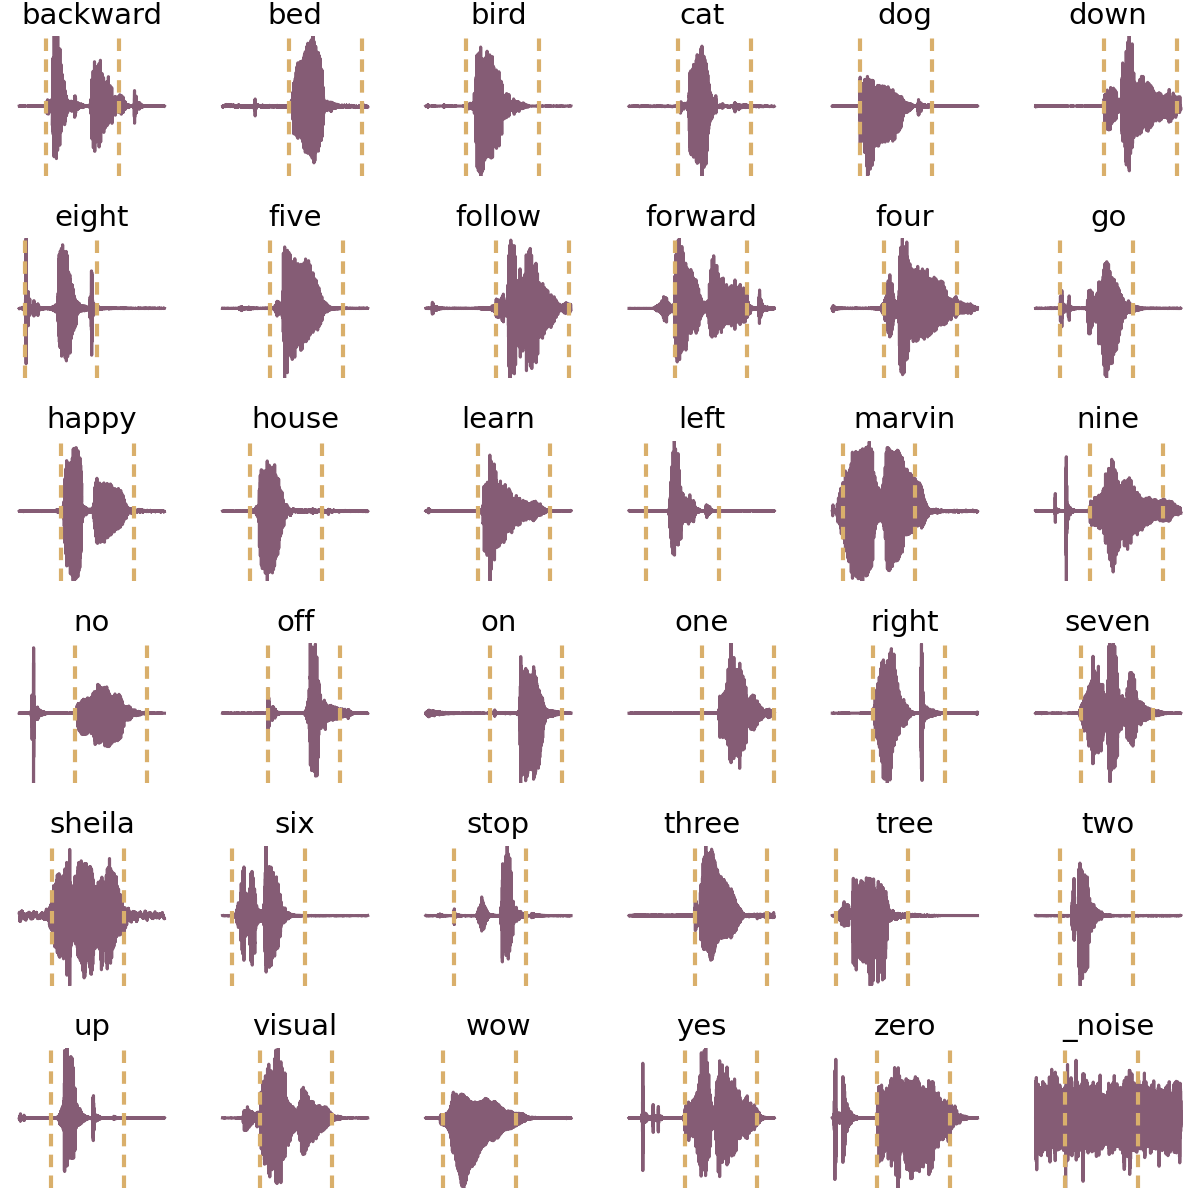
\includegraphics[width=0.65\textwidth]{./5_exp/figs/exp_dataset_speech_cmd_wav_grid.png}
  \caption{One random sample of each individual speech command in the speech commands dataset presented in normalized audio waveform.}
  \label{fig:exp_dataset_speech_cmd_wav_grid}
\end{figure}
\FloatBarrier
\noindent


% --
% statistics

\subsubsection{Observations of all available Examples in the Dataset}
Two histograms were created to observe the quality of all recorded files in the dataset.
Those histograms present an energy measure and a count of the sample length for each file.
The energy of a recorded file is an indicator for too silent or too loud (overdrive distortions) examples.
In the first version of the speech commands dataset, namely \texttt{v0.01}, silent files were a problem.
This had been fixed in the second version by rejecting those.
Therefore, the version \texttt{v0.01} is slightly more unclean than \texttt{v0.02}.
The energy value $e \in \R$ can be computed by
\begin{equation}\label{eq:exp_dataset_energy}
  e = \frac{1}{n} \left( \bm{x}^T \bm{x} \right),
\end{equation}
where $\bm{x} \in \R^n$ represents a single recorded file with a total number of $n$ samples.
The division through the sample length $n$ of each individual audio recording is required because not every file has a duration of \SI{1}{\second} (16000 samples).
For an unknown reason, many of the recordings consist of less than 16000 samples, which would be a problem if the sample length is too short to fully capture a keyword.
So the minimum duration of all examples was determined and found to last about \SI{0.4}{\second}.
This however, is adequate for words like \enquote{go}, where the reduced sample length often shows up.
\rfig{exp_dataset_hist} presents the mentioned histograms of all available examples in the dataset.
Note that the histograms are logarithmically (log) scaled.
\begin{figure}[!ht]
  \centering
    \subfigure[energy measure]{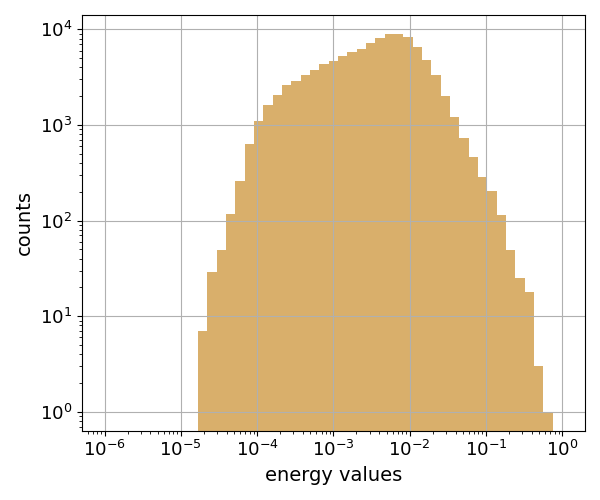
\includegraphics[width=0.42\textwidth]{./5_exp/figs/exp_dataset_hist_energy_overall.png}}
    \qquad
    \subfigure[count of sample length]{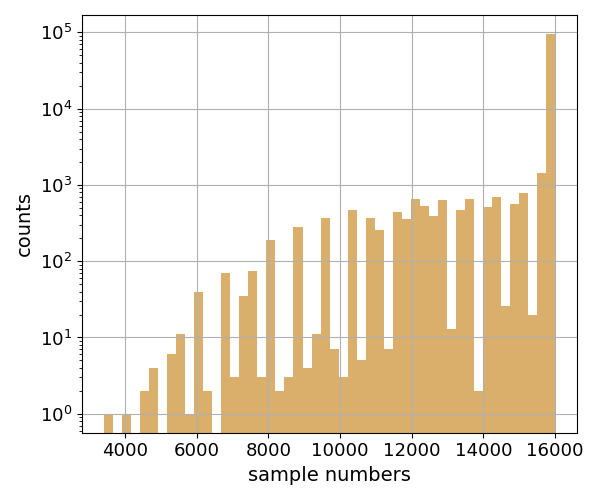
\includegraphics[width=0.42\textwidth]{./5_exp/figs/exp_dataset_hist_sample_overall.png}}
  \caption{Histograms of all available examples in the speech commands dataset \texttt{v0.02}, where one histogram shows an energy measure in log-log scale and the other a count of the sample length in log scale.}
  \label{fig:exp_dataset_hist}
\end{figure}
\FloatBarrier
\noindent
The histogram of the energy measure has one main lobe, which implies that there are no clusters of extremely silent or loud files.
For comparison, if silent files were extracted from the given background files, the energy of some of those would be in a range of $10^{-7} \dots 10^{-6}$.
The sample length histogram shows that most of the files consist of 16000 samples but many others have a smaller number of samples. 
This is relevant and has to be considered in the pre-processing of audio files, because input data to neural networks often have to be prepared to a fixed size if no sequential neural networks, such as Recurrent Neural Networks (RNNs), are used.


% --
% recording quality

\subsubsection{Recording Quality and Personal Experience}
The examples of the speech commands dataset \cite{Warden2018} were not recorded by professionals with high-end recording equipment.
In fact, the recordings had been done in an amateur kind of fashion so that the dataset is more suited to realistic environments intended for user applications.
This is also noted in the paper \cite{Warden2018}:
\begin{quote}
...This meant that the use of studio-captured samples seemed unrealistic, since that audio would lack background noise, would be captured with high-quality microphones, and in a formal setting. 
Successful models would need to cope with noisy environments, poor quality recording equipment, and people talking in a natural, chatty way...
\end{quote}
The recording devices of the speakers, who contributed examples to the dataset, were in most cases consumer microphones, as for instance, embedded microphones in laptops or mobile phones.

The conclusions drawn from listening to the examples in the dataset were as follows:
\begin{itemize}
  \item The quality of the examples in the dataset are ranging from excellent and perfectly recognizable to very poor, noisy, unrecognizable, and cut off. Although most of the examples are provided with sufficient quality.
  \item Different accents had been perceived, which suggests that people from several nationalities were involved.
  However, the bias is laid on American English, as noted in the paper.
  \item No children speakers were found.
\end{itemize}
Due to data privacy issues, the information on individual speakers is not displayed.
Therefore, it is not clear whether the dataset consists of an equal amount of male and female speakers and whether there are any children speakers included.
The last would be especially interesting for video games intended for children.

In many recordings, the background noise is imminent, such as traffic noise, chattering people, office sounds, and many more.
A quality check of the recorded files in the dataset had been done beforehand to ensure that poor quality examples are rejected.
Nevertheless, there are still some existing flaws, such as extremely loud or silent recordings, examples with inconsistent sample numbers, recordings that include too much noise or in the worst case noise only (very rarely), and cut off signals capturing only half of a word.
Those quality issues in the dataset can for most cases be neglected or fixed, such as inconsistent sample numbers. 
Other more problematic cases, like noise-only examples, should ideally be removed.
But since their occurrence is very rare it is not worth the effort.
Besides, it is usually not a problem for neural networks to cope with noisy datasets.
In many cases it is favorable when a dataset contains many noisy samples so that neural networks can learn invariance against noise, loudness differences, and other nuisances during training.
Moreover, if the training dataset is sufficiently large, and the test and validation sets do not contain very poor examples, there should be no problem in the training and evaluation of different models.
Finally, it has to be acknowledged that the dataset is published under the creative common license, hence it is freely available for everyone.


% --
% dataset structure

\subsubsection{Dataset Structure}\label{sec:exp_dataset_structure}
The speech command examples are stored in separate folders, which are named after each individual keyword.
The folder \texttt{\_background\_noise\_} contains six different background noise files, such as \texttt{white\_noise.wav} or \texttt{doing\_the\_dishes.wav}, with a duration of more than one minute each and altogether summing up to a duration of about \SI{400}{s}.
To extract noise examples from those files with a sufficient number of examples of over 3500, those noise files have to be extracted by a striding window of \SI{1}{\second} length shifted by \SI{0.110}{\second}.
The noise examples were assigned to the label \enquote{\_noise}.

Each waveform file from the keyword folders is named with an 8-digit hexadecimal hash code for the speaker identification and followed by the utterance number, for instance, \texttt{3b4f8f24\_nohash\_0.wav}.
With the speaker identification code known, it is possible to distinguish between different speakers.
However, as mentioned above, no further information about the speakers is provided due to data privacy issues.

Moreover, the dataset contains a testing file list called \texttt{testing\_list.txt} and a validation file list \texttt{validation\_list.txt}, where each row entry in the text files refer to a single file in the dataset, as for example \texttt{right/bb05582b\_nohash\_3.wav}.
The testing and validation file lists are applied in this thesis and the separation into sets are noted in \rtab{exp_dataset_all_labels}.


% --
% extracted examples

\subsubsection{Samples from the Feature Extraction}
The feature extracted data examples are stored to separate files before using them for training.
This has the practicability that features do not have to be extracted each time a new training instance of a neural network is performed.
\rfig{exp_dataset_speech_cmd_mfcc} visualizes samples from the extracted MFCCs with frame-based normalization.
\begin{figure}[!ht]
  \centering
    \subfigure[left]{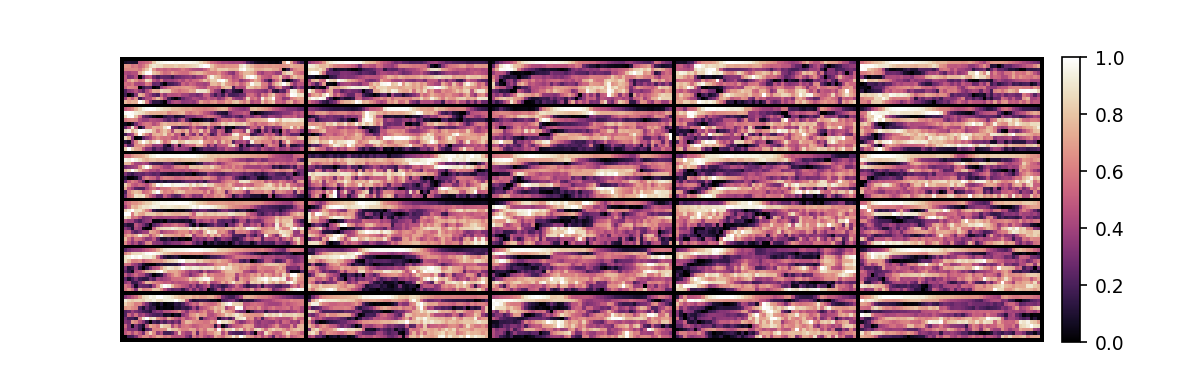
\includegraphics[width=0.48\textwidth]{./5_exp/figs/exp_dataset_speech_cmd_mfcc_left.png}}
    \subfigure[right]{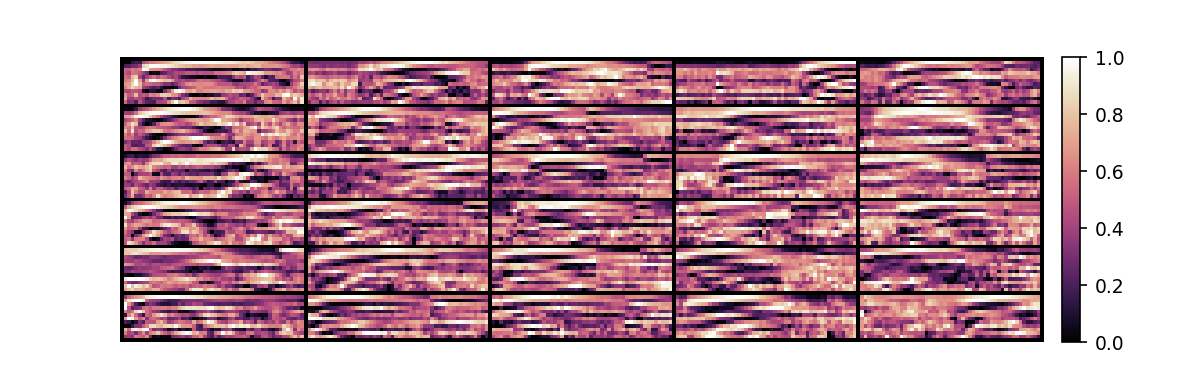
\includegraphics[width=0.48\textwidth]{./5_exp/figs/exp_dataset_speech_cmd_mfcc_right.png}}
    \subfigure[up]{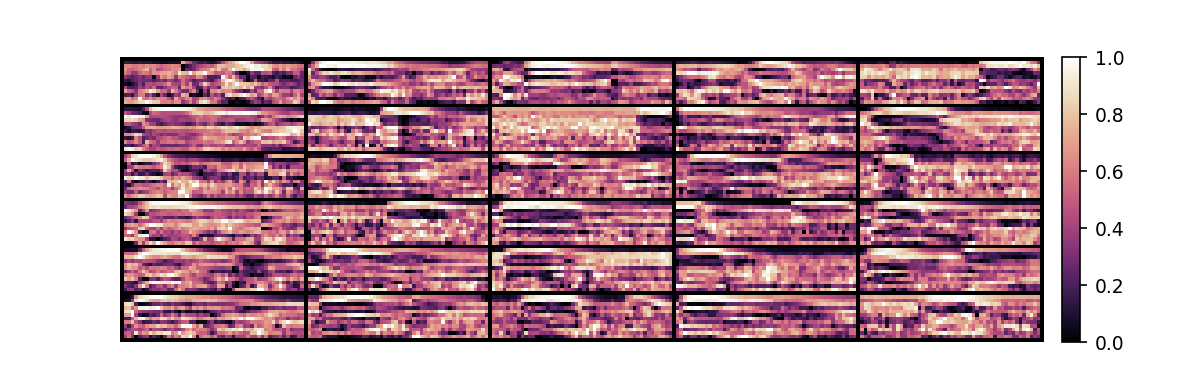
\includegraphics[width=0.48\textwidth]{./5_exp/figs/exp_dataset_speech_cmd_mfcc_up.png}}
    \subfigure[down]{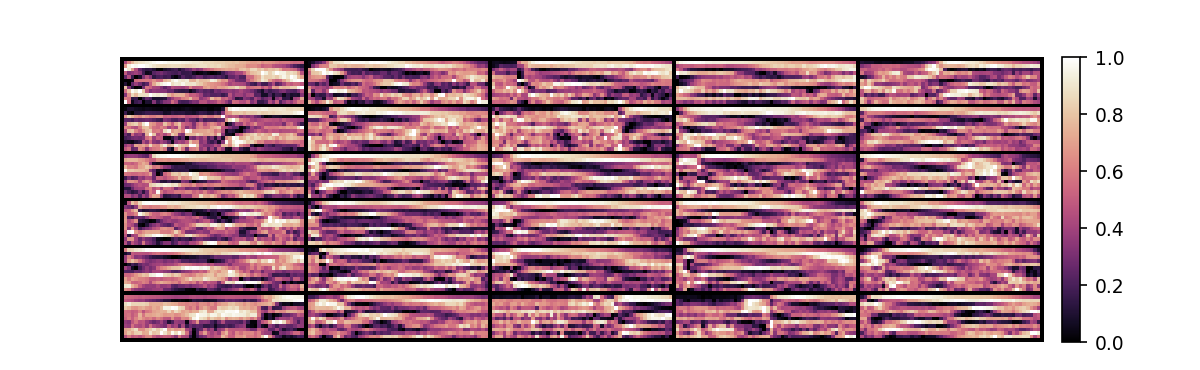
\includegraphics[width=0.48\textwidth]{./5_exp/figs/exp_dataset_speech_cmd_mfcc_down.png}}
    \subfigure[go]{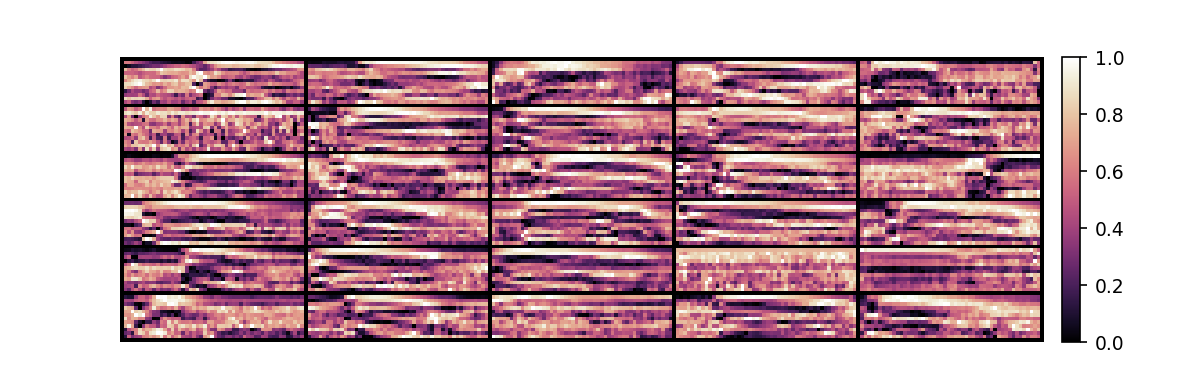
\includegraphics[width=0.48\textwidth]{./5_exp/figs/exp_dataset_speech_cmd_mfcc_go.png}}
  \caption{MFCC extraction of randomly selected 30 samples per class label obtained from the training set of the speech commands dataset \texttt{v0.02}. The corresponding class labels are written below the plots.}
  \label{fig:exp_dataset_speech_cmd_mfcc}
\end{figure}
\FloatBarrier
\noindent


% --
% my dataset

\subsection{My Dataset}\label{sec:exp_dataset_my}
The \enquote{my dataset} was created by the author of this thesis and contains five examples of each of the following keywords \{\enquote{left}, \enquote{right}, \enquote{up}, \enquote{down} and \enquote{go}\}.
The datasets purpose is mainly to have an additional test set for evaluating trained models on the authors own voice.
The examples per keyword are spoken with different emphasis and stress on individual phonemes for each keyword.
Also the prolongation of the words are different, for instance, in one example the word is spoken hasty and in the other sluggishly.
The emphasis and prolongation of the individual examples of keywords should ensure the diversity of the dataset.
It is relevant to mention that none of the self recorded files were used within the training set so that the neural networks performance is evaluated on unseen data.
\rfig{exp_dataset_my_wav_grid} illustrates all examples of the \enquote{my dataset} in raw audio waveform.
\begin{figure}[!ht]
  \centering
    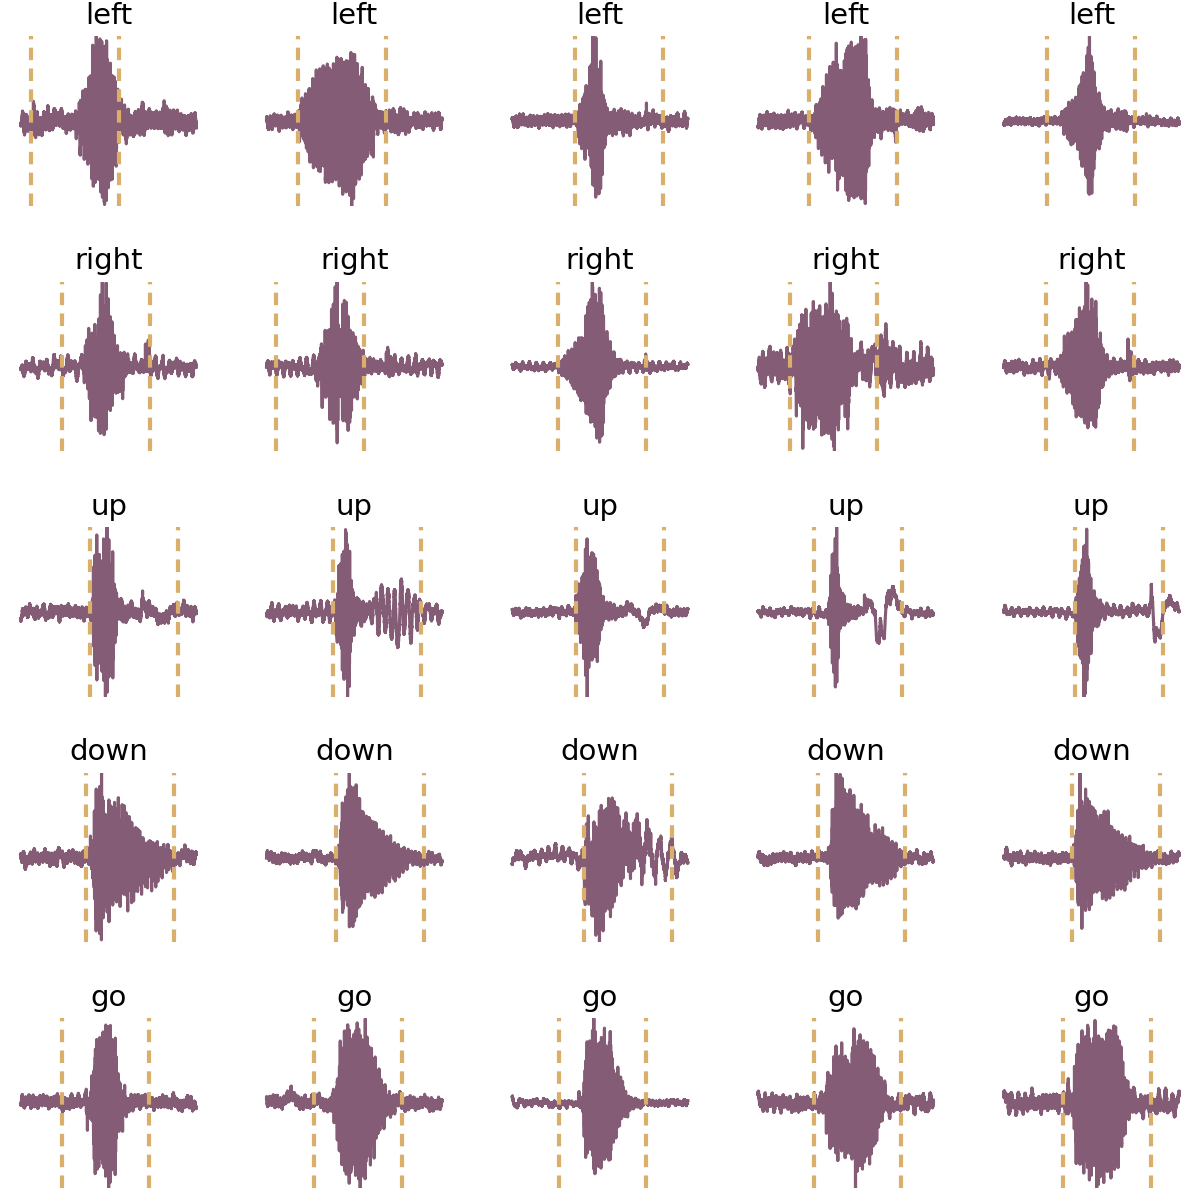
\includegraphics[width=0.6\textwidth]{./5_exp/figs/exp_dataset_my_wav_grid.png}
  \caption{Self recorded files of the \enquote{my dataset} in raw audio waveform.}
  \label{fig:exp_dataset_my_wav_grid}
\end{figure}
\FloatBarrier
\noindent
The same examples extracted to MFCC features are visualized in \rfig{exp_dataset_my_mfcc}.
\begin{figure}[!ht]
  \centering
    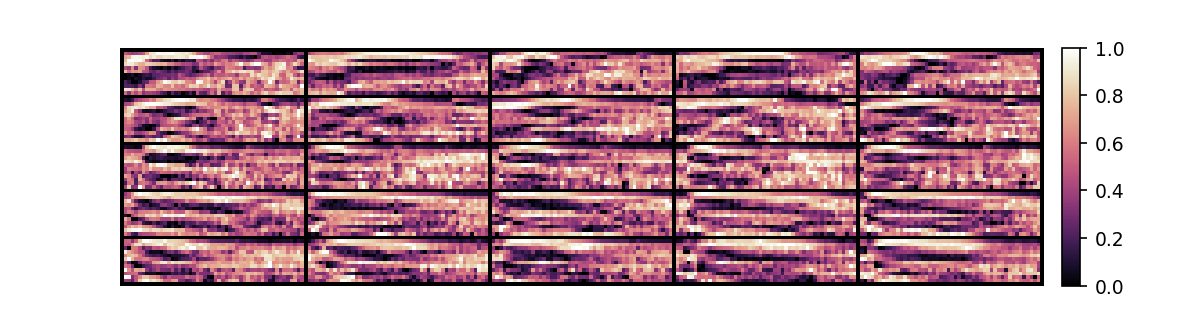
\includegraphics[width=0.65\textwidth]{./5_exp/figs/exp_dataset_my_mfcc.png}
  \caption{All MFCC extracted samples of the \enquote{my dataset} with the same ordering as shown in \rfig{exp_dataset_my_wav_grid}.}
  \label{fig:exp_dataset_my_mfcc}
\end{figure}
\FloatBarrier
\noindent
It turned out that it is a very hard task for neural networks to achieve a \SI{100}{\percent} classification accuracy upon the \enquote{my dataset} despite the fact that all examples were produced by the same speaker.
This is slightly worrying because acoustically each of the examples per word is perfectly distinguishable for humans.
For instance, in the classification of the five examples of \enquote{left}, the trained models may classify 4 examples as \enquote{left} and one as \enquote{right}.
It is difficult to examine why exactly this single example is wrongly classified.


% --
% preparation for neural networks

\subsection{Data Preparation for Neural Networks}\label{sec:exp_data_prep}
The neural network architectures are trained through supervised learning.
This implies that a class label $y_i \in \{0, 1, \dots, L - 1\}$ correspondence to each data example $x_i \in \mathcal{X}$ exists, where $L$ is the total number of classes and $\mathcal{X}$ is the input space of the data example.
The input space for MFCC features is, for example, $\mathcal{X} = \R^{C \times M}$ with $C$ cepstral coefficients and $M$ frames.
Selected examples including their labels form a set $S$ that can be used for training or testing, such as
\begin{equation}\label{eq:exp_dataset}
  S = \{ (x_i, y_i) \mid i = 0, 1, \dots, n - 1 \},
\end{equation}
where $n$ is the total number of examples within this set.
Class labels $y_i$ are usually translated to integer numbers that refer to indices in a class dictionary (enumerated vocabulary).
For instance, the label $y_1 = 0$ of example $i=1$ refers to the label \enquote{left} in the class dictionary \{0: \enquote{left}, 1: \enquote{right}\}.
It is essential that the enumeration of class labels in the class dictionary starts from zero because they should correspond to the output nodes in the used neural network.

\rsec{signal_mfcc} already showed how to extract MFCC features.
Nevertheless, it is important that each individual $x_i$ for all $i$ has the same dimension $\mathcal{X}$ so that a data preparation for the training of neural networks is possible.
It could happen that the sample numbers of the waveform files are inconsistent, as described in \rsec{exp_dataset_speech_cmd}, and therefore different dimension of individual data examples may be obtained.
To ensure that all $x_i$ have the same dimension, the audio files were adjusted to the same fixed sample length of a duration of \SI{1}{\second} and sampling frequency \SI{16}{\kilo\hertz}.
This was achieved by zero-padding the signals to the desired fixed length of $n = 16000$ samples.
Furthermore, a dither noise was added to ensure that neural networks are not confused when operating on pure zeros that emerge from the zero-padding of the data examples.
Additive White Gaussian Noise (AWGN) is applied to each data examples by
\begin{equation}\label{eq:exp_dither}
  \bm{x} = \bm{\tilde{x}} + \bm{v}, \quad \bm{v} \sim \mathcal{N}(\mu=0, \sigma=0.5 \cdot \tilde{x}_{quant}),
\end{equation}
where $\bm{v} \in \R^n$ is sampled from the normal distribution $\mathcal{N}$ with standard deviation given by the half of the quantization error $\tilde{x}_{quant} \in \R$, and $\bm{\tilde{x}} \in \R^n$ is the data example that is additionally zero-padded if its total sample number is less than 16000.
The quantization error $\tilde{x}_{quant}$ corresponds to the minimum of all absolute values from the samples of $\bm{\tilde{x}}$, except the pure zero entries added through zero-padding.
When the dithering is applied to the signal, the pure zeros are overwritten by the sampled dither noise while at the same time a minimal altering of the original signal is achieved.